\section{Ingeniería concurrente y de sistemas}
\begin{enumerate}
    \item Ingeniería concurrente (CE): Es un enfoque sistematizado para el diseño concurrente de productos y procesos, considerando desde el inicio todos los elementos que componen el ciclo de vida del producto. 

    Principales objetivos
    Incrementar la calidad del producto, la reducción general del gasto y la reducción del tiempo de desarrollo. 
    Principales características
    
    \begin{itemize}
        \item Mejor definición del problema de diseño 
        \item Implementación de herramientas de manufactura y ensamble en la etapa de diseño
        \item Mejora de la estimación del costo
        \item Reducción de problemas entre los procesos de diseño y manufactura
    \end{itemize}

    \item Ingeniería de sistemas: Consiste en el desarrollo de sistemas que sean capaces de satisfacer requerimientos dentro de un conjunto de restricciones bien definidas.
    
    Sistema: Es un conjunto o colección de diferentes elementos que en conjunto producen resultados que no se podrían obtener de forma independiente.

    Modelo TTDSE (Traditional Top-Down System Engineering) 
    Se compone de dos etapas principales
    
    \begin{itemize}
        \item S1: Análisis de necesidades, definición del sistema, definición de subsistemas, definición de componentes y definición de configuración de componentes.
        \item S2: Verificación desde la configuración de componentes al sistema final, validación y aprobando los resultados obtenidos. (modelo V)
    \end{itemize}
    
    \begin{figure}[h!]
        \centering
            \includegraphics[scale=0.25]{Proyecto Integrador Figuras/01 Modelo v.png}
            \caption{Modelo V}
    \end{figure}
    
    Modelo espiral: Consiste de cuatro procesos
    
    \begin{itemize}
        \item Planificación: investigación 
        \item Análisis y evaluación de riesgos: diseño y prototipo
        \item Desarrollo y pruebas
        \item Aprobación: mantenimiento, retroalimentación 
    \end{itemize}

    \begin{figure}[h!]
    \centering
        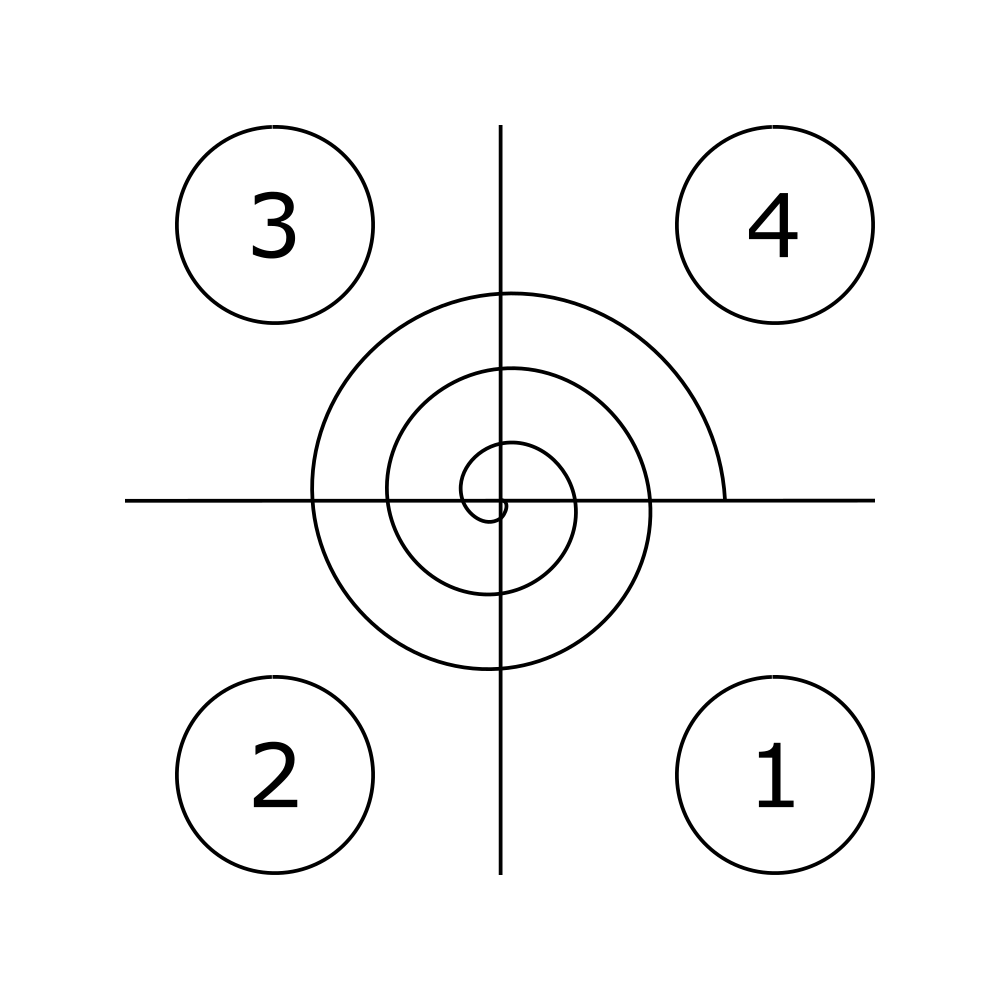
\includegraphics[scale=0.30]{Proyecto Integrador Figuras/02 Modelo Espiral.png}
        \caption{Modelo en espiral}
    \end{figure}

    Existen tres tipos de arquitecturas para sistemas
    
    \begin{itemize}
        \item A1: Arquitectura funcional-lógica\\
            Define que es lo que el sistema debe hacer, las acciones o funciones del sistema. Incluye modelos de información, procesos y el comportamiento inicial. (Modos de operación)
        \item A2: Arquitectura física
            Define los componentes, ensambles y elementos físicos que se requieren para el cumplimiento de las funciones, también representa las conexiones físicas entre componentes, sistemas, subsistemas y elementos.
        \item A3: Arquitectura de asignación
            Es el mapeo o relación de funciones y recursos necesarios. Se define el modelo final de comportamiento del sistema.
    \end{itemize}
\end{enumerate}

\begin{figure}[h!]
    \centering
        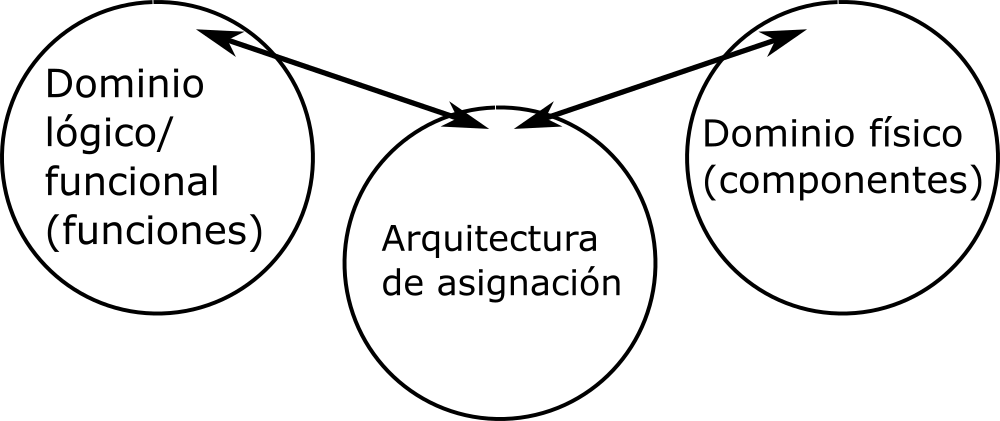
\includegraphics[scale=0.30]{Proyecto Integrador Figuras/03 Arquitectura de asignacion.png}
        \caption{Arquitectura de asignación}
\end{figure}

\begin{figure}[h!]
    \centering
        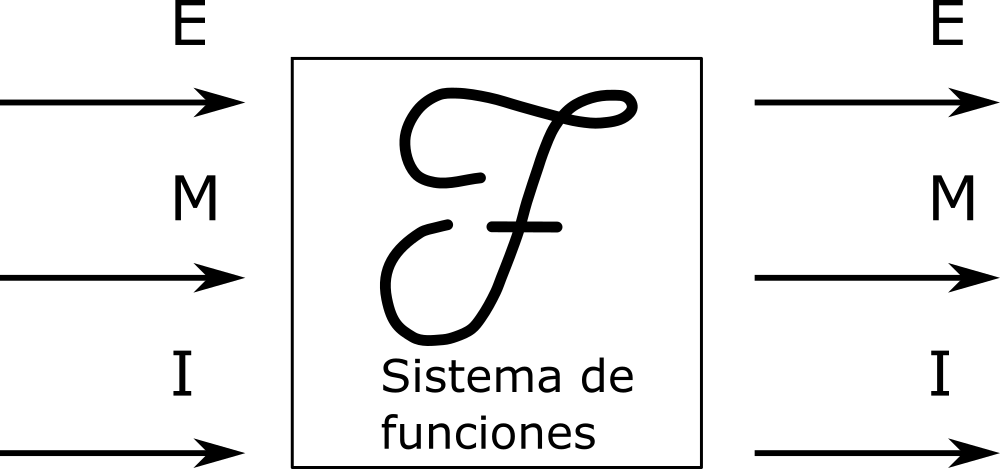
\includegraphics[scale=0.30]{Proyecto Integrador Figuras/04 Sistema de funciones.png}
        \caption{Sistema de funciones}
\end{figure}